\documentclass[12pt,a4paper]{article}

% --- Layout (brief: 12 pt, 1.5 line spacing, numbered headings) ---
\usepackage[a4paper,margin=25mm]{geometry}
\usepackage{setspace}
\usepackage{times}
\usepackage[T1]{fontenc}
\usepackage[utf8]{inputenc}
\usepackage{microtype}

% --- Figures, tables, maths ---
\usepackage{graphicx}
\usepackage{tikz}
\usetikzlibrary{positioning,arrows.meta,shapes.geometric,fit,calc}
\usepackage{booktabs}
\usepackage{tabularx}
\usepackage{longtable}
\usepackage{array}
\usepackage{amsmath,amssymb}
\usepackage{pdflscape}
\usepackage{caption}
\usepackage{float}
\usepackage{enumitem}
\usepackage{xcolor}
\definecolor{navy}{HTML}{0B2545}
\definecolor{teal}{HTML}{2A9D8F}
\definecolor{crimson}{HTML}{C0392B}
\definecolor{amber}{HTML}{E76F51}
\usepackage{fancyhdr}
\usepackage[round,authoryear]{natbib}
\usepackage{hyperref}

\graphicspath{{figures/}}
\onehalfspacing
\setcounter{tocdepth}{2}
\hypersetup{
  colorlinks=true,
  linkcolor=black,
  citecolor=black,
  urlcolor=blue
}

\pagestyle{fancy}
\setlength{\headheight}{15pt}
\fancyhf{}
\fancyhead[L]{\small 3004ENG --- Project Management Principles}
\fancyhead[R]{\small Group 1 --- Assessment 3}
\fancyfoot[C]{\thepage}
\renewcommand{\headrulewidth}{0.4pt}
\renewcommand{\tabularxcolumn}[1]{>{\raggedright\arraybackslash}p{#1}}

% Empty headings are otherwise glued together by LaTeX's \@nobreak
% (which is what produced the ~600 pt overfull vbox on the first compile).
\newcommand{\emptysec}{\par\mbox{}\par}
\numberwithin{table}{section}
\numberwithin{figure}{section}

% =============================================================================
\begin{document}

% -----------------------------------------------------------------------------
% Title page
% -----------------------------------------------------------------------------
\begin{titlepage}
\thispagestyle{empty}
\hypersetup{pageanchor=false}
\centering
\singlespacing
{\large Griffith School of Engineering and Built Environment}\\[0.25em]
{\large Griffith University}\\[1.2em]
{\LARGE\bfseries 3004ENG --- Project Management Principles}\\[0.5em]
{\Large Trimester 2, 2026}\\[1.1em]
{\LARGE\bfseries Eris TestFlight2 Launch Campaign}\\[0.35em]
{\Large Project Execution Plan}\\[0.7em]
{\large Assessment 3: Group Project Execution Plan --- Group 1}\\[1.1em]

\begin{tabular}{@{}ll@{}}
\textbf{Course} & 3004ENG Project Management Principles \\
\textbf{School} & Engineering and Built Environment \\
\textbf{Version} & Draft \\
\textbf{Submission date} & 2 October 2026 \\
\textbf{Word count} & \textit{(to be inserted; target 6{,}000 $\pm$ 10\%)} \\
\end{tabular}

\vspace{1.2em}

{\large\bfseries Project team}\\[0.5em]
\renewcommand{\arraystretch}{1.3}
\small
\begin{tabularx}{\textwidth}{@{}l l l >{\raggedright\arraybackslash}X r@{}}
\toprule
\textbf{Name} & \textbf{Student ID} & \textbf{Discipline} & \textbf{Project role} & \textbf{\%} \\
\midrule
Abdul Wahab Obeid & s5303839 & Mechatronics Engineering & Project Lead \& Integration Manager & 25.0 \\
Hadi Alkhub       & s5331680 & Software Engineering     & Lead Planner \& Scope Manager & 25.0 \\
Ziyad Alahmari    & s5375826 & Mechanical \& Aviation   & Risk \& Quality Lead & 25.0 \\
Ilsa Hashmi       & s5310047 & Software Engineering     & Stakeholder \& Resource Lead & 25.0 \\
\midrule
 &  &  & \textbf{Total} & \textbf{100.0} \\
\bottomrule
\end{tabularx}

\vfill
{\small Acting as a project management consultancy engaged to deliver launch-site operations at Bowen Orbital Spaceport.}
\par
\end{titlepage}

\hypersetup{pageanchor=true}
\onehalfspacing
\renewcommand{\arraystretch}{1.0}

\newpage
{\singlespacing
\tableofcontents
\vspace{1.8em}
\listoffigures
\vspace{1.8em}
\listoftables
\par}
\newpage

% -----------------------------------------------------------------------------
\section{Executive summary}
\label{sec:exec}
\emptysec

% -----------------------------------------------------------------------------
\section{Refined project overview}
\label{sec:overview}

\subsection{Background and purpose}
\label{sec:overview-background}
\emptysec

\subsection{Scope}
\label{sec:overview-scope}
\emptysec

\subsection{Charter baseline versus PEP refinement}
\label{sec:overview-changes}
\emptysec

\subsection{Objectives and success criteria}
\label{sec:overview-objectives}
\emptysec

\subsection{Work breakdown structure}
\label{sec:overview-wbs}

The work breakdown structure in Figure~\ref{fig:wbs} is the 100\% rule applied to launch-site operations at Bowen Orbital Spaceport. Four Level-2 workstreams---campaign governance, pad logistics, pad testing, and flight/closeout---decompose into seventeen Level-3 packages. Every scheduled activity except A-100 maps to exactly one of those packages, and every dollar in Table~\ref{tab:wbs-cost} sits in exactly one of them. A-100 is annotated beside the tree rather than inside it: the vehicle receipt window is an external zero-dollar wait that starts when out-of-scope freight reaches the gate. It belongs on the network because it drives stacking (A-122), but it is not a cost account.

Package 1.2.1 is one cost account with two schedule bars (A-121 site mobilisation and A-122 receiving inspection) because receiving cannot start until both the cleanroom and the vehicle exist. The remaining sixteen Level-3 codes are one-to-one with Table~\ref{tab:precedence}. Factory manufacture, engine research and development, and line-haul to the receiving gate are excluded.

The 7~August charter does not contain a notice to proceed for field work. Permitting (A-113) and Juru mobilisation (A-114) start on 10~August because those clocks have to run before hot fire. Physical pad occupancy before Gate~1 (A-111, 2~October) is a PEP choice, not a charter clause. What Gate~1 locks is the cost and schedule baseline.

\begin{figure}[H]
\centering
\resizebox{\textwidth}{!}{%
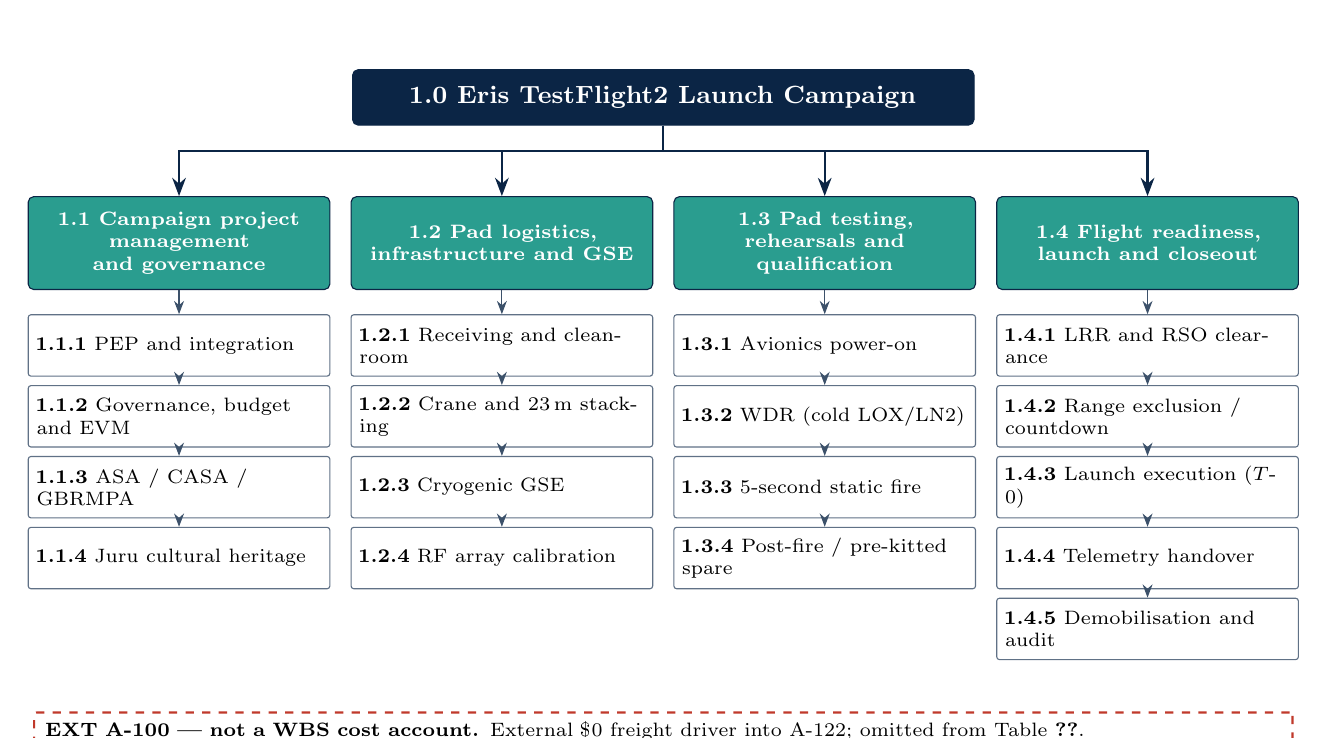
\begin{tikzpicture}[
  font=\sffamily,
  >=Stealth,
  L1/.style={draw=navy, fill=navy, text=white, rounded corners=2pt,
    inner xsep=7pt, inner ysep=6pt, font=\bfseries\small, align=center, text width=7.4cm},
  L2/.style={draw=navy, fill=teal, text=white, rounded corners=2pt,
    inner xsep=3pt, inner ysep=4pt, font=\bfseries\scriptsize, align=center,
    text width=3.62cm, minimum height=1.18cm},
  L3/.style={draw=navy!65, fill=white, rounded corners=1pt,
    inner xsep=3pt, inner ysep=2.4pt, font=\scriptsize, align=left,
    text width=3.62cm, minimum height=0.78cm},
  EXT/.style={draw=crimson, dashed, thick, rounded corners=1pt, fill=white,
    inner xsep=4pt, inner ysep=3.5pt, font=\scriptsize, align=left, text width=15.7cm}
]
\node[L1] (root) {1.0 Eris TestFlight2 Launch Campaign};

\node[L2] (n11) at (-6.15,-1.85) {1.1 Campaign project\\management and governance};
\node[L2] (n12) at (-2.05,-1.85) {1.2 Pad logistics,\\infrastructure and GSE};
\node[L2] (n13) at ( 2.05,-1.85) {1.3 Pad testing,\\rehearsals and qualification};
\node[L2] (n14) at ( 6.15,-1.85) {1.4 Flight readiness,\\launch and closeout};

\foreach \p in {n11,n12,n13,n14}
  \draw[navy, thick, ->] (root.south) -- ++(0,-0.32) -| (\p.north);

\node[L3] (n111) at (-6.15,-3.15) {\textbf{1.1.1} PEP and integration};
\node[L3] (n112) at (-6.15,-4.05) {\textbf{1.1.2} Governance, budget and EVM};
\node[L3] (n113) at (-6.15,-4.95) {\textbf{1.1.3} ASA / CASA / GBRMPA};
\node[L3] (n114) at (-6.15,-5.85) {\textbf{1.1.4} Juru cultural heritage};

\node[L3] (n121) at (-2.05,-3.15) {\textbf{1.2.1} Receiving and cleanroom};
\node[L3] (n122) at (-2.05,-4.05) {\textbf{1.2.2} Crane and 23\,m stacking};
\node[L3] (n123) at (-2.05,-4.95) {\textbf{1.2.3} Cryogenic GSE};
\node[L3] (n124) at (-2.05,-5.85) {\textbf{1.2.4} RF array calibration};

\node[L3] (n131) at ( 2.05,-3.15) {\textbf{1.3.1} Avionics power-on};
\node[L3] (n132) at ( 2.05,-4.05) {\textbf{1.3.2} WDR (cold LOX/LN2)};
\node[L3] (n133) at ( 2.05,-4.95) {\textbf{1.3.3} 5-second static fire};
\node[L3] (n134) at ( 2.05,-5.85) {\textbf{1.3.4} Post-fire / pre-kitted spare};

\node[L3] (n141) at ( 6.15,-3.15) {\textbf{1.4.1} LRR and RSO clearance};
\node[L3] (n142) at ( 6.15,-4.05) {\textbf{1.4.2} Range exclusion / countdown};
\node[L3] (n143) at ( 6.15,-4.95) {\textbf{1.4.3} Launch execution ($T$-0)};
\node[L3] (n144) at ( 6.15,-5.85) {\textbf{1.4.4} Telemetry handover};
\node[L3] (n145) at ( 6.15,-6.75) {\textbf{1.4.5} Demobilisation and audit};

\foreach \a/\b in {n11/n111,n111/n112,n112/n113,n113/n114,
                   n12/n121,n121/n122,n122/n123,n123/n124,
                   n13/n131,n131/n132,n132/n133,n133/n134,
                   n14/n141,n141/n142,n142/n143,n143/n144,n144/n145}
  \draw[navy!80, ->] (\a.south) -- (\b.north);

\node[EXT] (a100) at (0,-8.05) {%
  \textbf{EXT A-100 --- not a WBS cost account.} External \$0 freight driver into A-122; omitted from Table~\ref{tab:wbs-cost}.};

\end{tikzpicture}%
}
\caption[Work breakdown structure]{Work breakdown structure for Eris TestFlight2 launch-site operations. Seventeen Level-3 packages are the cost accounts in Table~\ref{tab:wbs-cost}. A-100 is an external schedule bar, not a seventeenth-plus cost line.}
\label{fig:wbs}
\end{figure}


% -----------------------------------------------------------------------------
\section{Schedule management}
\label{sec:schedule}

The campaign schedule turns the WBS into a dated baseline for board approval. Dates come from a finish-to-start activity-on-node network. The pad calendar is seven days a week from 10~August to 1~December~2026, because LOX load, static fire and lift-off do not stop for weekends. Approved lift-off ($T$-0) stays 15~November~2026. That day still sits inside the charter's last-allowed window of Q1~2027. A five-day pull-in to 10~November exists only if R-14 is realised (ASA flight authorisation or a CASA NOTAM refuses the 15~November slot). It is not the baseline.

\subsection{Network logic and float analysis}
\label{sec:schedule-network}

Links are finish-to-start with zero lag, drawn activity-on-node. Textbook discrete-time notation writes $EF = ES + D$ when $EF$ is exclusive. Every date on the Bowen calendar is inclusive. The identities used here are
\begin{equation}
ES_{i} = \max_{j \in P_{i}}(EF_{j}) + 1,
\qquad
EF_{i} = ES_{i} + D_{i} - 1,
\label{eq:fwd}
\end{equation}
\begin{equation}
LF_{i} = \min_{k \in S_{i}}(LS_{k}) - 1,
\qquad
LS_{i} = LF_{i} - D_{i} + 1,
\label{eq:bwd}
\end{equation}
$P_{i}$ and $S_{i}$ are the predecessor and successor sets of activity $i$. Where $P_{i}$ is empty, $ES$ is the campaign start. Total float and free float are
\begin{equation}
TF_{i} = LS_{i} - ES_{i} = LF_{i} - EF_{i},
\qquad
FF_{i} = \min_{k \in S_{i}}(ES_{k}) - EF_{i} - 1,
\label{eq:float}
\end{equation}
If $S_{i}$ is empty, $FF_{i} = TF_{i}$. Launch-critical means $TF_{i} = 0$ on a path that sets $T$-0 or closeout. Table~\ref{tab:precedence} is the full pass. It matches the locked register.

The forward pass gives two $TF = 0$ chains. They stay independent until hot fire. The vehicle path starts at the external \$0 freight wait (A-100; not a Gilmour launch-critical bar). Receiving (A-122) follows, then stacking (A-123), Wet Dress Rehearsal (A-132) and static fire (A-133). The permit path is ASA / CASA / GBRMPA permits (A-113) into static fire. RF calibration (A-125) is a finish-to-start predecessor of static fire, so the array is live before hot fire. It is not launch-critical. After static fire the tail from post-fire diagnostics (A-134) through closeout (A-145) is one critical chain. The PEP lock (A-111) finishes on 2~October by an imposed Must-Finish-On (Gate~1). It is not launch-critical. The Week~4 charter approved the document, not field mobilisation.

The paths meet in two staged merges. Wet Dress Rehearsal waits on stacking, cryogenic GSE (A-124), avionics power-on (A-131) and Juru monitors (A-114). That is the technical merge. Static fire then waits on the rehearsal, flight permits \emph{and} RF calibration. That is the regulatory and range-instrument merge. Launch Readiness Review (LRR, A-141) waits on post-fire diagnostics, not on static fire. Signing that flight-clearance gate on incomplete hot-fire data would break the hold-point logic of an AS9100D system \citep{sae2016}.

Feeder float is not interchangeable. Avionics has one day into the rehearsal. Cryogenic GSE has three. RF calibration has 39 days. It sits in August--September so it does not sit on the October pad peak. Moving it does not change 15~November. Cleanroom mobilisation (A-121) has $TF = 3$ but $FF = 0$, so delay is absorbed before $T$-0 only by consuming the GSE float. Total float protects $T$-0. Free float protects the successor. Figure~\ref{fig:network_logic} draws the links.

\begin{figure}[H]
\centering
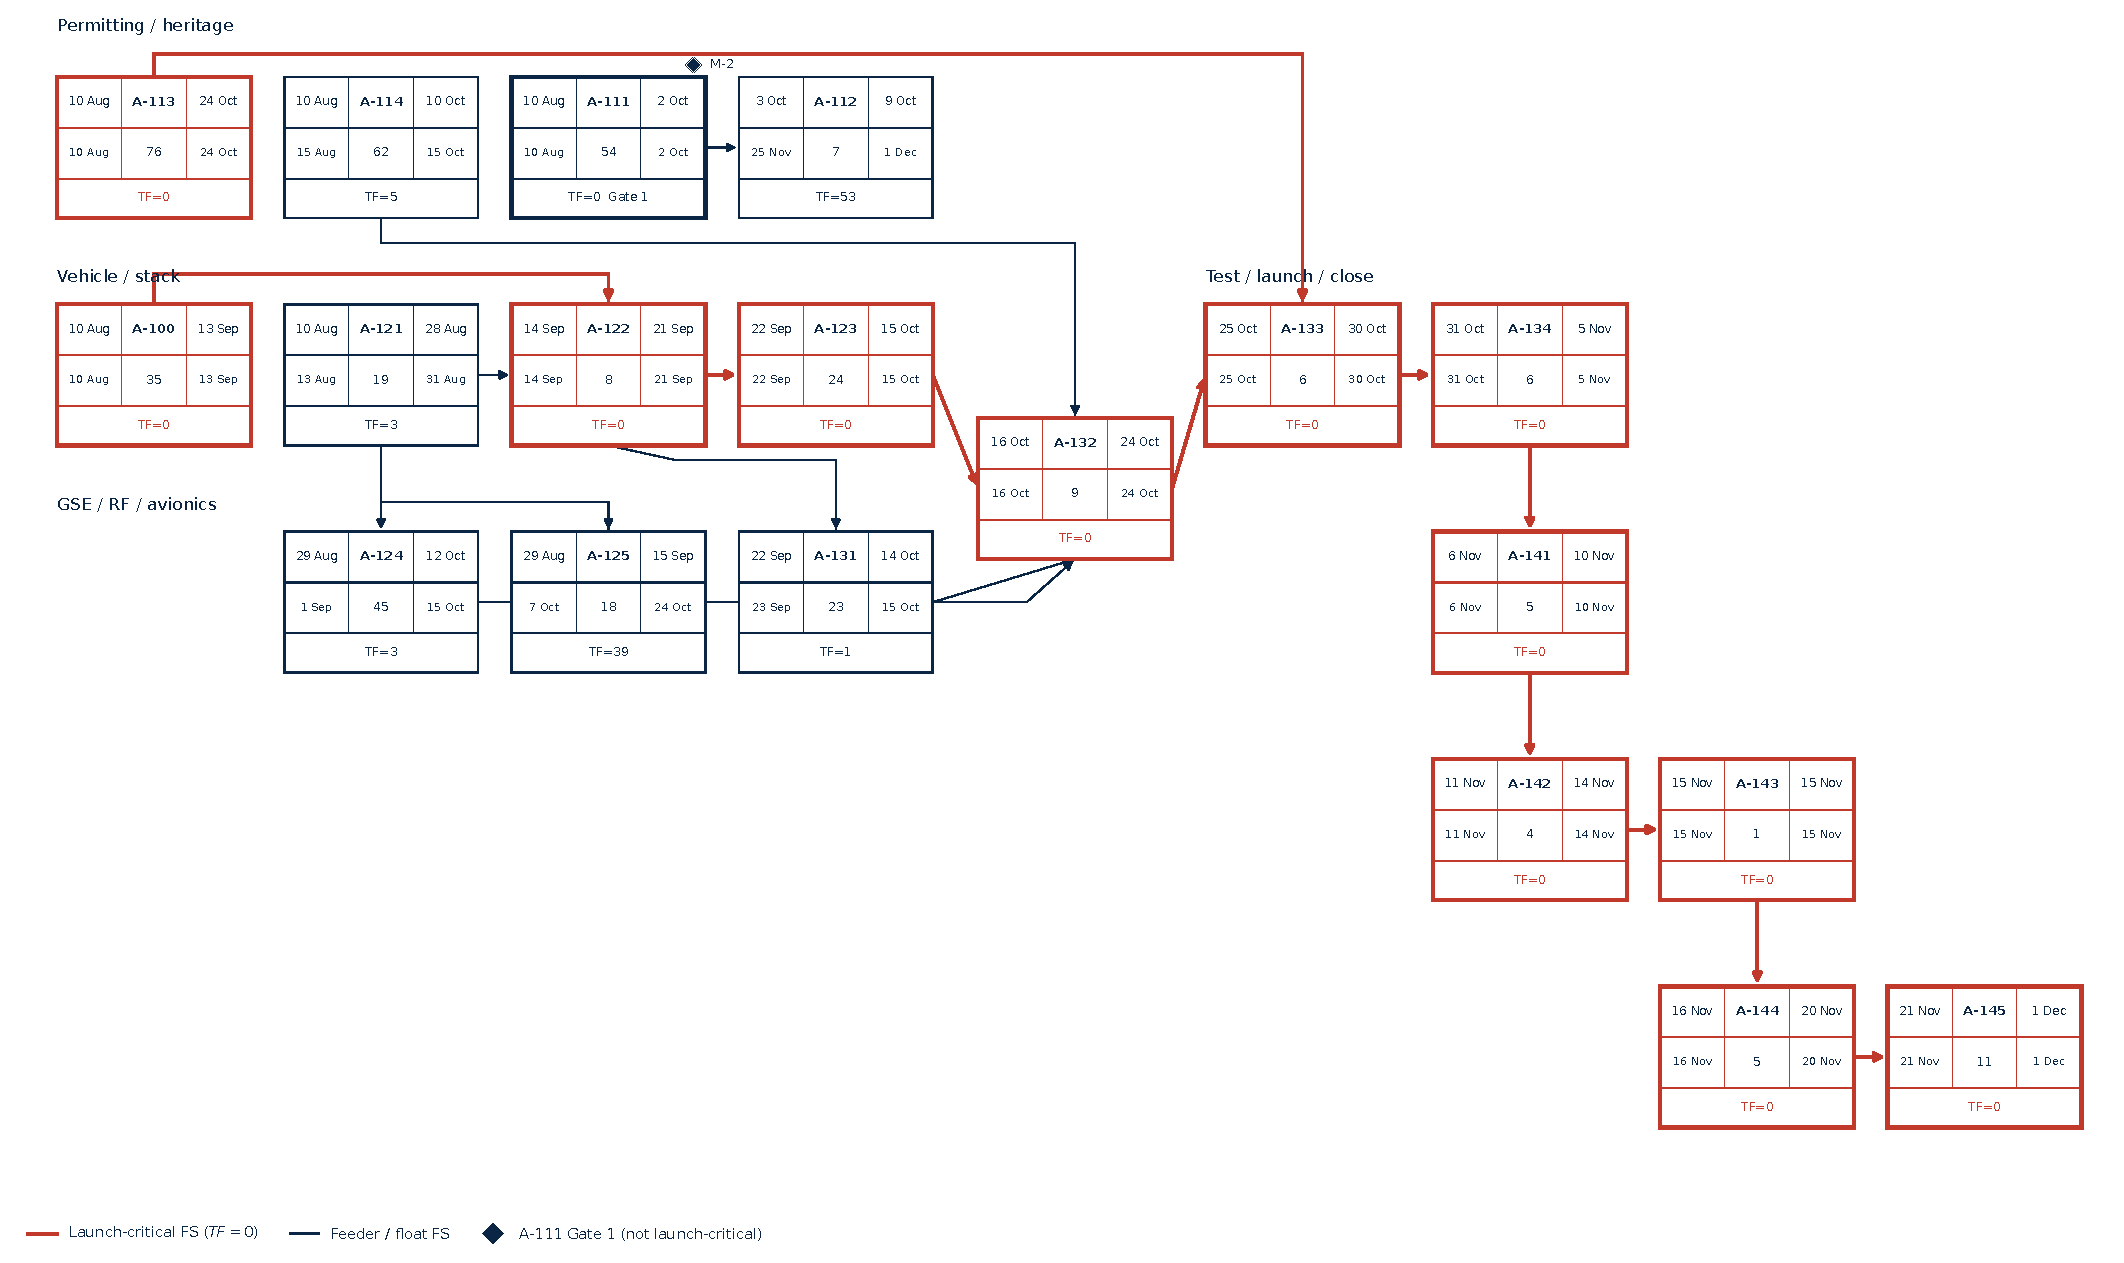
\includegraphics[width=\linewidth]{network_logic.pdf}
\caption[Activity-on-node network]{Activity-on-node network for the Bowen campaign. Node bands are $ES$ / ID / $EF$, $LS$ / duration / $LF$, and $TF$. Crimson arrows are launch-critical finish-to-start links. The vehicle path and the permit path merge at static fire; RF calibration is the labelled south-routed feeder into the same merge; LRR waits on post-fire diagnostics, not on static fire. The PEP lock is Gate-1 constrained and is not launch-critical. Freight receipt is a grey dashed external \$0 driver, not a crimson Gilmour bar.}
\label{fig:network_logic}
\end{figure}

\begin{landscape}
\small
\setlength{\tabcolsep}{4.2pt}
\renewcommand{\arraystretch}{1.15}
\begin{longtable}{@{}l l l r l c c c c r r c@{}}
\caption[Activity precedence and float register]{Master campaign activity precedence and float register. Dates are inclusive. $FF = \min(ES_{\text{succ}}) - EF - 1$ days, or $FF = TF$ if there is no successor. The PEP lock $TF = 0$ is an imposed Gate~1 finish, not launch-critical. The freight wait $TF = 0$ is an external pin (CP $=$ Ext), not a Gilmour launch-critical bar.}
\label{tab:precedence}\\
\toprule
ID & WBS & Activity & $D$ & Pred. & ES & EF & LS & LF & TF & FF & CP \\
\midrule
\endfirsthead
\caption[]{Master campaign activity precedence and float register (continued).}\\
\toprule
ID & WBS & Activity & $D$ & Pred. & ES & EF & LS & LF & TF & FF & CP \\
\midrule
\endhead
\bottomrule
\endfoot
A-100 & EXT & Vehicle receipt (external driver) & 35 & --- & 10 Aug & 13 Sep & 10 Aug & 13 Sep & 0 & 0 & Ext \\
A-111 & 1.1.1 & PEP and integration baseline & 54 & --- & 10 Aug & 2 Oct & 10 Aug & 2 Oct & 0* & 0 & Gate \\
A-112 & 1.1.2 & EVM control stand-up & 7 & A-111 & 3 Oct & 9 Oct & 25 Nov & 1 Dec & 53 & 53 & N \\
A-113 & 1.1.3 & ASA / CASA / GBRMPA permits & 76 & --- & 10 Aug & 24 Oct & 10 Aug & 24 Oct & 0 & 0 & Y \\
A-114 & 1.1.4 & Juru monitor mobilisation & 62 & --- & 10 Aug & 10 Oct & 15 Aug & 15 Oct & 5 & 5 & N \\
A-121 & 1.2.1a & Site mobilisation and cleanroom & 19 & --- & 10 Aug & 28 Aug & 13 Aug & 31 Aug & 3 & 0 & N \\
A-122 & 1.2.1b & Receiving and unpacking & 8 & A-100, A-121 & 14 Sep & 21 Sep & 14 Sep & 21 Sep & 0 & 0 & Y \\
A-123 & 1.2.2 & Crane and vertical stacking & 24 & A-122 & 22 Sep & 15 Oct & 22 Sep & 15 Oct & 0 & 0 & Y \\
A-124 & 1.2.3 & Cryo GSE piping and checkouts & 45 & A-121 & 29 Aug & 12 Oct & 1 Sep & 15 Oct & 3 & 3 & N \\
A-125 & 1.2.4 & RF telemetry calibration & 18 & A-121 & 29 Aug & 15 Sep & 7 Oct & 24 Oct & 39 & 39 & N \\
A-131 & 1.3.1 & Avionics power-on sweeps & 23 & A-122 & 22 Sep & 14 Oct & 23 Sep & 15 Oct & 1 & 1 & N \\
A-132 & 1.3.2 & Wet Dress Rehearsal (cold) & 9 & A-114, A-123, A-124, A-131 & 16 Oct & 24 Oct & 16 Oct & 24 Oct & 0 & 0 & Y \\
A-133 & 1.3.3 & 5-second static fire & 6 & A-132, A-113, A-125 & 25 Oct & 30 Oct & 25 Oct & 30 Oct & 0 & 0 & Y \\
A-134 & 1.3.4 & Post-fire / pre-kitted spare & 6 & A-133 & 31 Oct & 5 Nov & 31 Oct & 5 Nov & 0 & 0 & Y \\
A-141 & 1.4.1 & LRR and RSO clearance & 5 & A-134 & 6 Nov & 10 Nov & 6 Nov & 10 Nov & 0 & 0 & Y \\
A-142 & 1.4.2 & Range exclusion and countdown & 4 & A-141 & 11 Nov & 14 Nov & 11 Nov & 14 Nov & 0 & 0 & Y \\
A-143 & 1.4.3 & Launch execution ($T$-0) & 1 & A-142 & 15 Nov & 15 Nov & 15 Nov & 15 Nov & 0 & 0 & Y \\
A-144 & 1.4.4 & Telemetry decrypt and handover & 5 & A-143 & 16 Nov & 20 Nov & 16 Nov & 20 Nov & 0 & 0 & Y \\
A-145 & 1.4.5 & Demobilisation and closeout & 11 & A-144 & 21 Nov & 1 Dec & 21 Nov & 1 Dec & 0 & 0 & Y \\
\end{longtable}
\end{landscape}

\subsection{Schedule baseline, Gantt visualisation and milestone integrity}
\label{sec:schedule-baseline}

The dates in Table~\ref{tab:precedence} \emph{are} the schedule baseline. Figure~\ref{fig:gantt_chart} plots the same $ES$/$EF$ values. Launch-critical bars are crimson. Remaining total float is a teal whisker to $LF$. Permitting, heritage, mobilisation and GSE run through August and September. October is the physical peak: stacking 15~October, WDR 16--24~October, static fire 25--30~October. November is the flight-clearance tail.

Two Week~4 collisions are closed here. The charter dated pad integration 15~October in Objective~1 and stacking as M-4 on 28~October. The PEP locks M-4 to stacking on \textbf{15~October~2026}. That restores the cold-flow window before hot fire. Handover ``within five days of lift-off'' was also dated M-8 at 22~November, seven days after a 15~November $T$-0. M-8 is now telemetry handover on \textbf{20~November}. The facility licence is already held, so permits gate static fire, not stacking. Treating flight permits as a stacking predecessor was an initiation error.

Three gates sit on the baseline. Gate~1 is the PEP lock on 2~October. Gate~2 is permits on 24~October. Without those instruments static fire cannot start. That path is already $TF = 0$. Gate~3 is LRR on 10~November. Crashing stacking without crashing the permit path therefore cannot pull $T$-0.

\begin{figure}[!htbp]
\centering
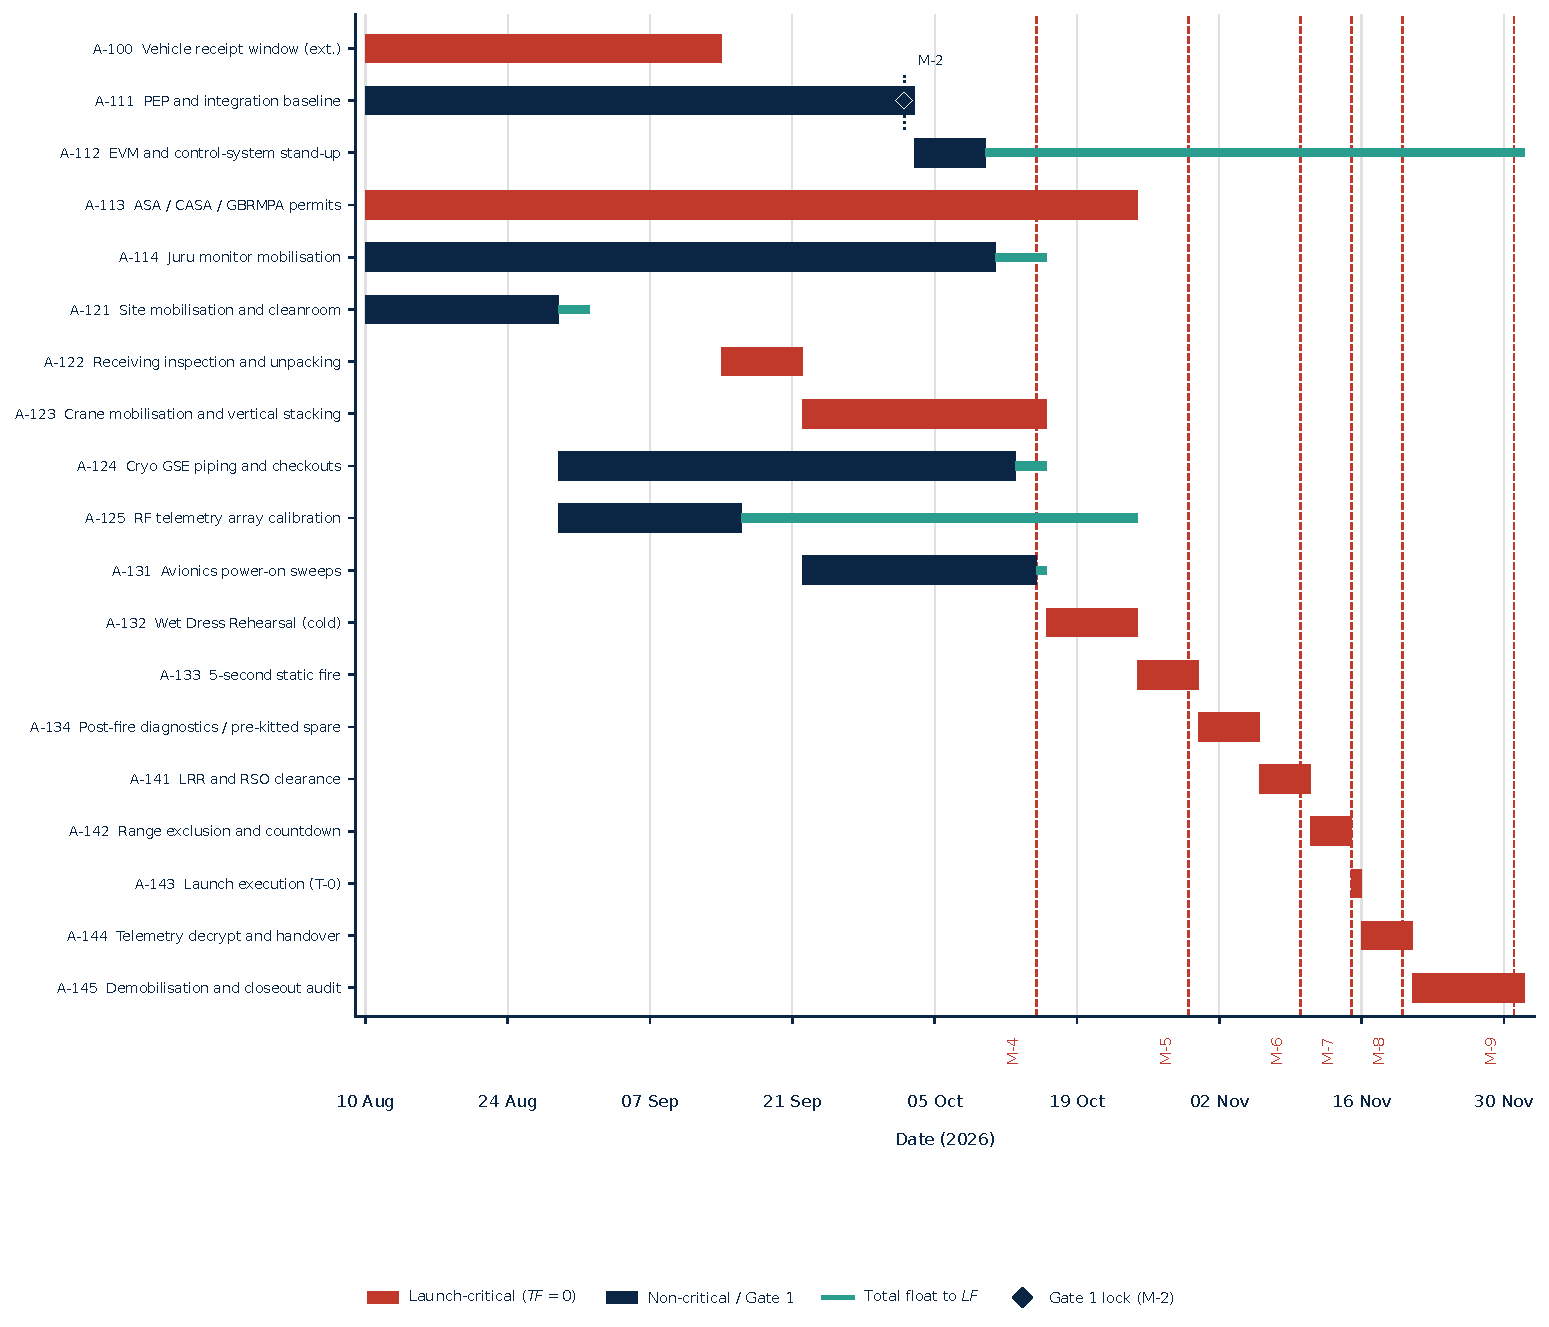
\includegraphics[width=\linewidth]{gantt_chart.pdf}
\caption[Baseline Gantt chart]{Baseline Gantt from 10~August to 1~December~2026, plotted from the same $ES$/$EF$ values as Table~\ref{tab:precedence}. Crimson bars are launch-critical. The hatched grey bar is the external \$0 freight wait. Teal whiskers show total float to $LF$. Vertical markers are M-2 (navy, Gate~1) and M-4 through M-9. Option~C is not drawn on this baseline.}
\label{fig:gantt_chart}
\end{figure}

\subsection{Schedule compression: crashing and fast-tracking}
\label{sec:schedule-compression}

Fast-tracking overlaps sequential work, usually at zero direct cost. Crashing adds resource on critical work and is paid as a cost slope. The Board question is whether $T$-0 can move from 15~November to 10~November if R-14 is realised (ASA / CASA refuses the 15~November slot). Five days must come off a $TF = 0$ path that actually sets lift-off. After the static-fire merge that path is the tail from diagnostics through lift-off. Crashing stacking by five days saves \textbf{zero} days on $T$-0 while permits still finish on 24~October. Overlapping stacking with cryogenic GSE also saves zero days. GSE already runs in parallel with stacking.

The crash-cost slope on a crashed activity is
\begin{equation}
\text{Cost slope} = \frac{\Delta C}{\Delta T}
= \frac{\text{crash cost} - \text{normal cost}}{\text{normal duration} - \text{crash duration}}.
\label{eq:slope}
\end{equation}
Table~\ref{tab:compression} and Figure~\ref{fig:compression_curve} compare three options that each claim five days. Only Option~C is both CPM-valid and acceptable against the LRR hold.

\begin{table}[H]
\centering
\small
\setlength{\tabcolsep}{3.5pt}
\caption[Schedule compression evaluation]{Schedule compression evaluation. All three options save five days on $T$-0 if they work as drawn. Baseline $T$-0 stays 15~November. Option~C is a draw on the \$78{,}890 reserve if R-14 fires, not an addition to the \$1{,}500{,}000 base.}
\label{tab:compression}
\begin{tabularx}{\textwidth}{@{}l >{\raggedright\arraybackslash}X c r r >{\raggedright\arraybackslash}X l@{}}
\toprule
Option & Activities modified & Days & Added cost & Slope & Secondary risks & Verdict \\
\midrule
A Pure fast-track & Diagnostics $\to$ LRR SS+1 (review overlaps diagnostics) & 5 & \$0 & \$0/d & Review before diagnostic close-out; LRU rework; AS9100D hold-point failure & Rejected \\
B Pure crash & Diagnostics crashed 6~$\to$~1~d & 5 & \$40{,}000 & \$8{,}000/d & Fatigue; skipped thermal/electrical screens; recycle into LRR & Rejected \\
C Hybrid (if R-14 fires) & Diagnostics 6~$\to$~1~d extra labour (\$21{,}000); LRR kept at 5~d; countdown kept at 4~d & 5 & \textbf{\$21{,}000} & \textbf{\$4{,}200/d} & Screens kept; R-15 4~d marine hold intact & Contingent \\
\bottomrule
\end{tabularx}
\end{table}

Decision: baseline $T$-0 stays 15~November. If R-14 fires, the Board draws Option~C and lift-off moves to 10~November. That is the only option that is valid on the network and acceptable on quality.

Option~A is a pure fast-track. It buys five days at \$0 by starting the review one day after diagnostics start. The review board would sit while those diagnostics were still open. AS9100D is the quality rule this campaign uses for hold points \citep{sae2016}. The LRR hold (HP-4) is sign-off of that review. A hold point is a stop: the next job cannot start until the planned checks are done and the hold is released. Option~A would let flight clearance start before post-fire data are complete. Signing that gate on incomplete data is a hold-point failure. Waiting to sign until diagnostics finish does not save five days; it creates rework. Fast-tracking the review is rejected.

Option~B is a pure crash. It compresses diagnostics from six days to one. The slope is $\$40{,}000/5 = \$8{,}000$ per day. A 24-hour diagnostic war room on a vehicle that has just fired is the work most likely to skip thermal and electrical screens. Crashing diagnostics without extra screens is rejected.

Option~C is the hybrid. It takes the five days only from diagnostics. Extra labour keeps the thermal and electrical screens that Option~B would skip: two specialists and two technicians for five days ($2\times\$165 + 2\times\$95 = \$520$/h $\times$ 8~h $=$ \$4{,}160/d, published as the same \$4{,}200/d unit used on the crawler) for \$21{,}000. The slope is $\$21{,}000/5 = \$4{,}200$ per day. Launch Readiness Review stays five days. Countdown stays four days, so the marine hold on R-15 is not consumed. If invoked, diagnostics sit on 31~October only, the review on 1--5~November, countdown on 6--9~November, and lift-off on \textbf{10~November}. The \$21{,}000 is drawn from the \$78{,}890 contingency only if R-14 is realised. It is not loaded into the \$1{,}500{,}000 base. Figure~\ref{fig:gantt_chart} is not redrawn. Feeder floats do not tighten: avionics stays at $TF = 1$, cryogenic GSE at $TF = 3$.

Option~C is chosen because it is cheaper than Option~B (\$4{,}200/d not \$8{,}000/d), it keeps the LRR hold that Option~A would break, and crashing stacking cannot move $T$-0 while permits still finish on 24~October.

\begin{figure}[H]
\centering
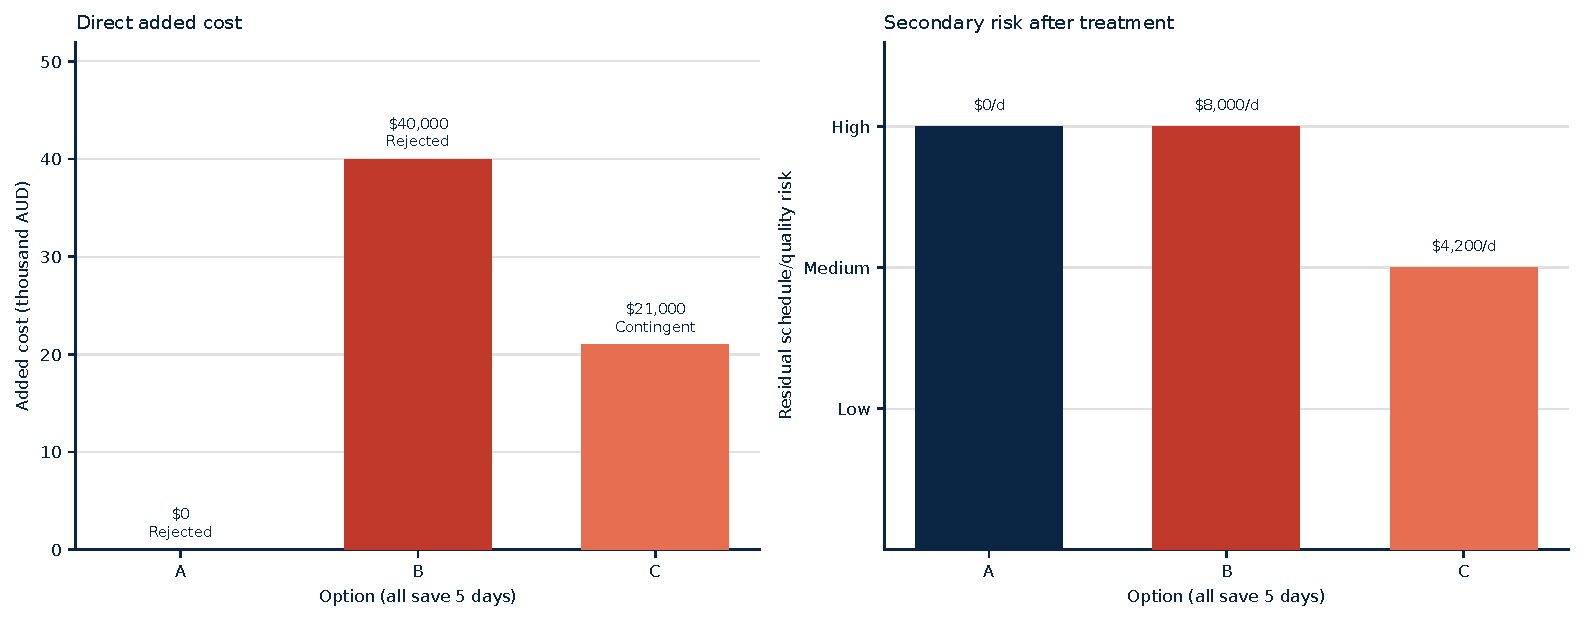
\includegraphics[width=0.98\linewidth]{compression_tradeoff.pdf}
\caption[Compression cost and risk trade-off]{Compression trade-off for a five-day pull-in of $T$-0. Left: direct added cost. Right: residual schedule and quality risk after treatment. Option~C is the only CPM-valid pull-in that keeps LRR at five days, countdown at four days, and pays \$4{,}200 per day rather than \$8{,}000.}
\label{fig:compression_curve}
\end{figure}


% -----------------------------------------------------------------------------
\section{Cost management}
\label{sec:cost}

The cost baseline is the WBS in Figure~\ref{fig:wbs} priced at Level~3. Seventeen control accounts sum to a work estimate of \$1{,}500{,}000. Contingency of \$78{,}890 is sized from residual expected monetary value plus four named residual items, not from a round-number markup, so the authorised budget at completion is \$1{,}578{,}890.

\subsection{Estimating basis and assumptions}
\label{sec:cost-basis}

The estimate is bottom-up at Level~3, with analogous plant and commodity rates beside the hours. Loaded 2026 Australian-dollar rates are used throughout: systems-engineering and project-management time at \$150/h, pad technicians at \$95/h, cryogenic and range-safety specialists at \$165/h, and surge technicians at \$100/h. The Manufacturing Award C10 ordinary hourly rate is \$29.45 from the first full pay period on or after 1~July~2026 \citep{fwc2026}. Charge-out is C10 multiplied by a named employment on-cost, then utilisation and overhead---the product is in the notes to Table~\ref{tab:wbs-cost}. Those factors do not change the \$1{,}500{,}000 lines. The 100~t crawler for 23\,m stacking is priced at \$4{,}200 per wet day, including operator, from published Queensland plant-hire schedules cross-checked against Rawlinsons \citep{rawlinsons2025}.

Inclusions are the seventeen packages in Figure~\ref{fig:wbs}: mobilisation through demobilisation at Bowen. Factory manufacture, engine research and development, and freight to the receiving gate remain out of scope, so A-100 is a zero-dollar external driver rather than a cost account. The four-person surge crew (\$22{,}400) is inside WBS~1.3.3 as planned capacity. The \$21{,}000 hybrid compression cost in Section~\ref{sec:schedule-compression} is a contingent draw against the \$78{,}890 reserve if R-14 is realised; it is not in the \$1{,}500{,}000 performance measurement baseline.

The 7~August charter does not authorise field spend. Permitting and Juru work start on 10~August because those durations must finish before hot fire. Other August--September pad cost is a PEP choice: planned value already on the clock by Gate~1 (A-111, 2~October) is \$602{,}301 (40.2\% of the work PMB), including stacking in progress. Gate~1 locks remaining spend; it does not pretend the campaign is only a mobilisation paper.

\subsection{WBS cost baseline}
\label{sec:cost-wbs}

Table~\ref{tab:wbs-cost} is the rollup. Pad logistics (1.2) is \$518{,}000 (34.5\% of the work estimate), pad testing (1.3) \$414{,}000 (27.6\%), governance (1.1) \$300{,}000 (20.0\%), and flight/closeout (1.4) \$268{,}000 (17.9\%).

\begin{table}[!htbp]
\centering
\footnotesize
\setlength{\tabcolsep}{4.2pt}
\caption[Bottom-up cost baseline by WBS]{Bottom-up cost baseline by Level-3 WBS package. Totals equal the work estimate of \$1{,}500{,}000. A-100 is omitted because it is not a cost account.}
\label{tab:wbs-cost}
\begin{tabularx}{\textwidth}{@{}l p{4.15cm} r X@{}}
\toprule
WBS & Package & Amount (AUD) & Basis \\
\midrule
1.1.1 & PEP and integration & 72{,}000 & 480~h PM @ \$150 \\
1.1.2 & Governance and EVM & 48{,}000 & 320~h planner/cost @ \$150 \\
1.1.3 & ASA / CASA / GBRMPA & 88{,}000 & ASA \$42k $+$ CASA \$28k $+$ GBRMPA \$18k \\
1.1.4 & Juru monitors and heritage & 92{,}000 & Two monitors + survey \\
1.2.1 & Receiving and cleanroom & 68{,}000 & Technician hours + consumables \\
1.2.2 & Crane and 23\,m stacking & 218{,}000 & 8 lift + 16 weld/NDT/bolt-up d $\times$ \$4{,}200 $=$ \$100{,}800 + riggers \\
1.2.3 & Cryo GSE & 180{,}000 & Valves/piping + specialist crew \\
1.2.4 & RF array calibration & 52{,}000 & Crew + analyser hire \\
1.3.1 & Avionics power-on & 58{,}000 & Engineers @ \$150/h + EGSE \\
1.3.2 & WDR (cold) & 160{,}000 & Includes bulk LOX 25~t and LN2 \$68{,}500 \\
1.3.3 & Static fire & 148{,}000 & Includes surge hire \$22{,}400 \\
1.3.4 & Post-fire / pre-kitted spare & 48{,}000 & Engineers + spare handling \\
1.4.1 & LRR and RSO & 38{,}000 & Review board; payload witnesses \\
1.4.2 & Range exclusion / marine & 58{,}000 & Patrol boats + NOTAM \\
1.4.3 & Launch and telemetry capture & 82{,}000 & Launch-day operations \\
1.4.4 & Decrypt and handover & 24{,}000 & Five-day engineering handover \\
1.4.5 & Demobilisation and audit & 66{,}000 & Site restore + audit \\
\midrule
\textbf{Base} & & \textbf{1{,}500{,}000} & \mbox{} \\
\bottomrule
\end{tabularx}

\vspace{0.35em}
{\footnotesize\textit{Notes.} Labour: MA000010 C10 ordinary \$29.45/h (ppc 1~July~2026) from Annual Wage Review 2026 \citep{fwc2026}. Employment on-cost $=$ super 12\% $+$ annual leave 7.69\% $+$ personal leave 3.85\% $+$ public holidays 4.23\% $+$ LSL 2.17\% $+$ 17.5\% leave loading on annual leave $+$ workers compensation (1.8\% professional / 4.5\% pad) $+$ QLD payroll tax 4.75\% ($1.378\times$ professional, $1.405\times$ pad). Charge-out then divides by utilisation and applies overhead, with no consultancy fee: engineer/PM $\$29.45 \times 1.378 / 0.72 \times 2.66 = \$150$; technician $\$29.45 \times 1.405 / 0.85 \times 1.95 = \$95$; specialist $\$29.45 \times 1.378 / 0.60 \times 2.44 = \$165$. Surge is C10 $\times$ 1.5 overtime $\times$ pad on-cost $/ 0.85 \times 1.37 = \$100$. Crane: 8 lift days and 16 weld/NDT/bolt-up days at the same wet \$4{,}200 (QLD 100~t crawler band about \$3{,}800--\$4{,}500/day), cross-checked against Rawlinsons \citep{rawlinsons2025}. Weather dollars sit only in RES (4 extra wet days). 1.1.3: ASA 280~h @ \$150 $=$ \$42{,}000; CASA CRIS airspace instrument \$28{,}000; GBRMPA permission \$18{,}000 \citep{asa2025,casa2024,gbrmpa2019}. LOX/LN2 \$68{,}500 is a bulk industrial-gas analogue inside 1.3.2. Surge \$22{,}400 $=$ $4 \times 7$~d $\times$ 8~h $\times$ \$100 and sits in 1.3.3, not in contingency.}
\end{table}

The largest package is crane mobilisation and stacking (1.2.2, \$218{,}000) because A-123 occupies 24 calendar days on the launch-critical path. The wet crawler is on hire for that whole window: 8 lift days and 16 weld, NDT and bolt-up days at \$4{,}200, which is \$100{,}800, with the balance in rigger labour. Those 16 days are plant duration, not weather. Weather dollars sit in one place only: RES four extra wet days at \$4{,}200 $=$ \$16{,}800. R-06 is a schedule control (dawn-lift window) with residual EMV \$0, so it is not a second crane line. Wet Dress Rehearsal (1.3.2) carries \$68{,}500 of bulk liquid oxygen and nitrogen inside \$160{,}000. Static fire (1.3.3) carries the planned surge inside \$148{,}000. The seventeen lines sum to \$1{,}500{,}000 with no miscellaneous remainder. Package 1.2.1 remains one control account for A-121 and A-122.

\subsection{Contingency}
\label{sec:cost-contingency}

Contingency is not a 15\% story. Table~\ref{tab:contingency} adds a residual expected-monetary-value pool to four named residual items. Treatments already sit in the \$1{,}500{,}000 base (surge hire, dawn-lift window, dual-path recorders, pre-kitted spare), so the pool uses residual $P'_{\%}\times I_{\$}$, not inherent $P_{\%}$. Summing the ten cost-bearing risks R-01, R-02, R-03, R-04, R-05, R-07, R-09, R-10, R-13 and R-14 gives \$35{,}760. The residual-uncertainty (RES) allowance is itemised in the same table and sums to \$43{,}130. Vehicle freight is out of scope and is not in RES. The two components sum to \$78{,}890, which is 5.26\% of \$1{,}500{,}000, and the authorised $BAC$ is therefore \$1{,}578{,}890.

\begin{table}[H]
\centering
\small
\caption[Contingency build-up]{Contingency build-up. The 5.26\% ratio is residual EMV plus four named residual items, not an input markup.}
\label{tab:contingency}
\begin{tabular}{@{}p{8.4cm} r p{4.1cm}@{}}
\toprule
Component & Amount (AUD) & Rule \\
\midrule
$\Sigma$ residual EMV of ten cost-bearing risks & 35{,}760 & Residual $P'_{\%}\times I_{\$}$; treatments already in the base \\
LOX/LN2 price variance (18\% of \$68{,}500 gases) & 12{,}330 & In-scope commodity; not freight \\
Crane weather (only weather \$): 4~d $\times$ \$4{,}200 & 16{,}800 & Extra wet days; R-06 is schedule-only \\
GN2/N2 purge: 40 G-size cylinders $\times$ \$200 & 8{,}000 & Named multiply-out \\
Cryogenic kit: 3 $\times$ 3~m LOX hoses $\times$ \$1{,}400 $+$ seal kit \$1{,}800 & 6{,}000 & Named multiply-out \\
\midrule
\textbf{RES subtotal} & \textbf{43{,}130} & Itemised; not a plug to 15\% \\
\textbf{Contingency reserve} & \textbf{78{,}890} & 5.26\% of base \\
\textbf{$BAC$} & \textbf{1{,}578{,}890} & Base + contingency \\
\bottomrule
\end{tabular}
\end{table}

Several register rows are kept out of the \$35{,}760 so that money is not counted twice. R-08 (pad-civil defect) is contract-transferred under the design-and-construct package and carries no Gilmour EMV. R-06, R-11, R-15, R-16, R-17 and R-18 are schedule or HSE exposures without a residual dollar draw. R-12 is the TestFlight~1 in-flight failure mode; the vehicle is factory product, so site-ops EMV is \$0. If R-14 is realised and Option~C is invoked, the \$21{,}000 is drawn from the \$78{,}890 reserve. It is not added to the \$1{,}500{,}000 work baseline. There is no management reserve above $BAC$: unknown unknowns would require a board variation this plan does not authorise.

\subsection{Time-phased budget and cash flow}
\label{sec:cost-cashflow}

The performance measurement baseline is the work estimate spread across the same dates as Table~\ref{tab:precedence}. Table~\ref{tab:cashflow} and Figure~\ref{fig:scurve} use a uniform daily burn on each activity. October is the peak month because stacking, Wet Dress Rehearsal and the five-second static fire all sit there. December is a residual on 1~December, not a parking place for unused contingency.

\begin{table}[H]
\centering
\small
\caption[Time-phased planned value]{Time-phased planned value of the \$1{,}500{,}000 work baseline. Contingency is not monthly spend.}
\label{tab:cashflow}
\begin{tabular}{@{}lrr@{}}
\toprule
Month & Period PV (AUD) & Cumulative PV (AUD) \\
\midrule
Aug 2026 & 155{,}951 & 155{,}951 \\
Sep 2026 & 407{,}188 & 563{,}139 \\
Oct 2026 (peak: stack, WDR, static fire) & 628{,}861 & 1{,}192{,}000 \\
Nov 2026 & 302{,}000 & 1{,}494{,}000 \\
Dec 2026 & 6{,}000 & \textbf{1{,}500{,}000} \\
\bottomrule
\end{tabular}
\end{table}

The S-curve therefore terminates at \$1{,}500{,}000. Figure~\ref{fig:scurve} draws $BAC = \$1{,}578{,}890$ as a horizontal authorisation line. Planned value at M-4 (15~October) is \$865{,}578---the same total used in Section~\ref{sec:delivery-evm}. Planned value at Gate~1 (2~October) is \$602{,}301. Option~C's \$21{,}000 is excluded from every period in Table~\ref{tab:cashflow}. If it is spent, it appears as actual cost charged to contingency, not as a rewrite of the S-curve.

\begin{figure}[H]
\centering
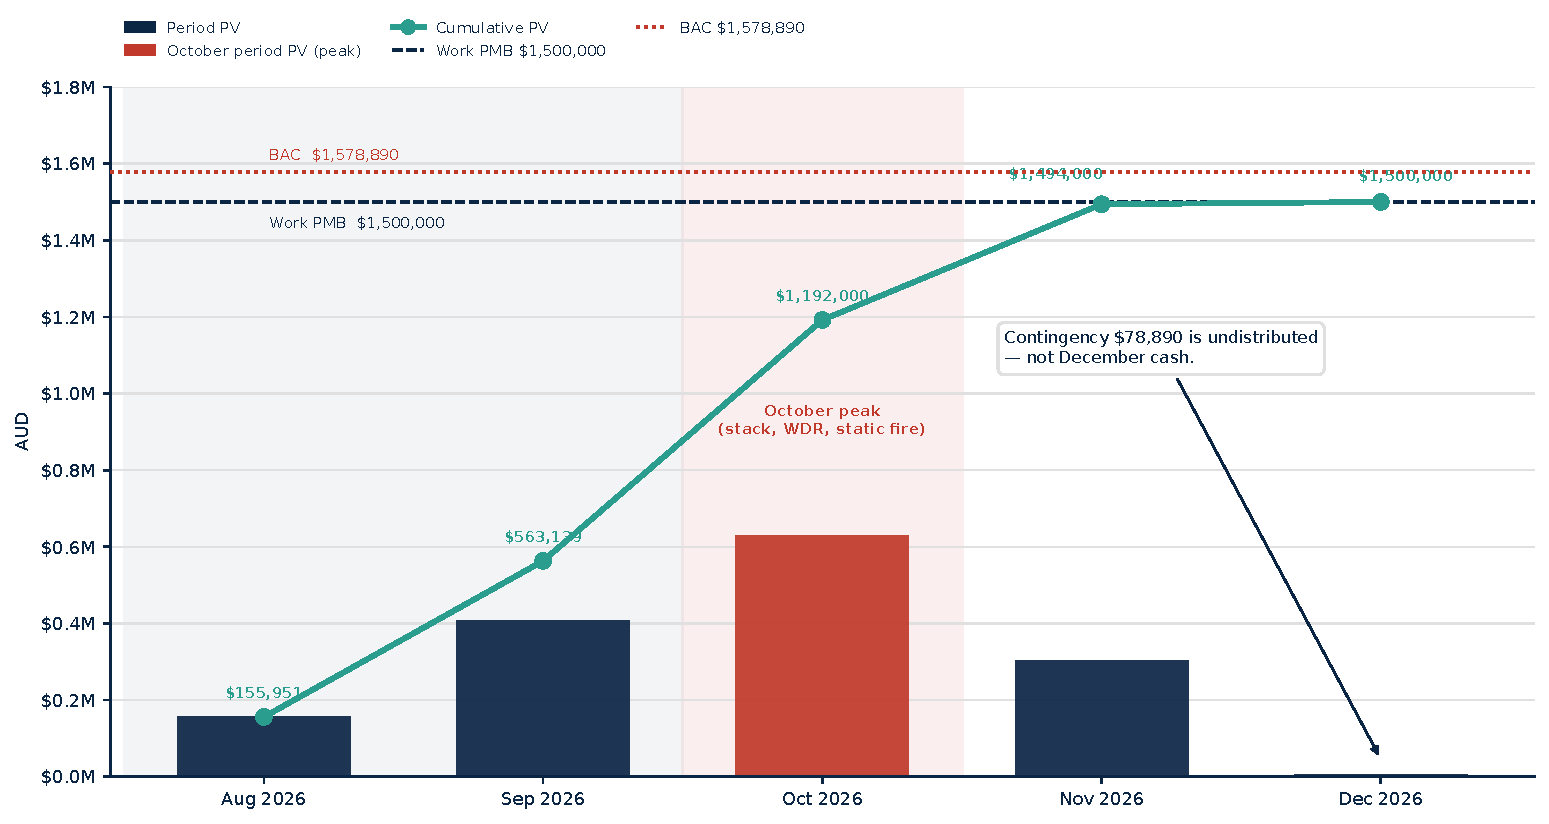
\includegraphics[width=0.98\linewidth]{cash_flow_scurve.pdf}
\caption[Planned-value S-curve]{Cumulative planned-value S-curve for the Bowen campaign. Period bars are monthly PV; the teal line is cumulative PV and ends at the \$1{,}500{,}000 work baseline. The crimson dotted line is $BAC$ (\$1{,}578{,}890) as an authorisation ceiling, not December cash. Contingency remains undistributed. Option~C is not in the curve.}
\label{fig:scurve}
\end{figure}


% -----------------------------------------------------------------------------
\section{Resource management}
\label{sec:resource}

Pad occupancy is a health-and-safety limit, not a roster convenience. The organic Bowen crew is eight certified technicians. The blast-zone, suit-air and access-control cap is twelve people. Eight is therefore the standing organisation; twelve is the occupancy ceiling that Figure~\ref{fig:resources} must never cross \citep{pmi2021,kerzner2017}.

\subsection{Roles and responsibilities}
\label{sec:resource-raci}

Accountability is split across two layers, with exactly one Accountable owner per Level-3 package in Table~\ref{tab:raci}. The consultancy layer is Abdul Wahab Obeid, Hadi Alkhub, Ziyad Alahmari and Ilsa Hashmi. The field layer is the Launch Director, Range Safety Officer, GSE Lead, Avionics Specialist, Juru Cultural Officer and the design-and-construct package manager. Consulted names must see the work product before the Accountable owner signs; they are not a second A.

The pattern matches the network. Hadi is Accountable for stacking because the dawn-lift window is a schedule control (R-06). Hot operations are Accountable to the Launch Director with the RSO consulted, except range exclusion, which the RSO owns. Closeout audit is Ziyad's, so quality is not marking its own homework.

\begin{table}[H]
\centering
\footnotesize
\setlength{\tabcolsep}{3.6pt}
\caption[RACI for Level-3 packages]{RACI for Level-3 packages. Exactly one Accountable owner per row. Field titles are as used on the pad; consultancy names are the Group~1 officers.}
\label{tab:raci}
\begin{tabularx}{\textwidth}{@{}l >{\raggedright\arraybackslash}p{3.15cm} >{\raggedright\arraybackslash}p{2.55cm} >{\raggedright\arraybackslash}p{2.35cm} X@{}}
\toprule
WBS & Package & A & R & C \\
\midrule
1.1.1 & PEP and integration & Abdul & Hadi & Ziyad, Ilsa \\
1.1.2 & Governance and EVM & Ilsa & Hadi & Abdul \\
1.1.3 & ASA / CASA / GBRMPA & Abdul & Hadi & Launch Director \\
1.1.4 & Juru heritage & Juru Officer & Ilsa & Abdul, Ziyad \\
1.2.1 & Receiving / cleanroom & GSE Lead & D\&C mgr & Hadi, Ilsa \\
1.2.2 & Crane and stacking & Hadi & GSE Lead & Launch Director, RSO \\
1.2.3 & Cryo GSE & D\&C mgr & GSE Lead & Ziyad \\
1.2.4 & RF calibration & Avionics & Hadi & Launch Director \\
1.3.1 & Avionics power-on & Avionics & GSE Lead & Hadi \\
1.3.2 & WDR (cold) & GSE Lead & Juru Officer & Ziyad, LD, RSO \\
1.3.3 & Static fire & Launch Director & GSE Lead & RSO, Ziyad, Avionics \\
1.3.4 & Post-fire / pre-kitted spare & Avionics & GSE Lead & Ziyad \\
1.4.1 & LRR and RSO & Launch Director & RSO & Abdul, Ziyad, Juru Officer, payload sponsor \\
1.4.2 & Range exclusion & RSO & Launch Director & Juru Officer \\
1.4.3 & Launch ($T$-0) & Launch Director & RSO, Avionics & Abdul \\
1.4.4 & Telemetry handover & Avionics & Hadi & Ilsa \\
1.4.5 & Demob and audit & Ziyad & D\&C mgr & Ilsa, Abdul \\
\bottomrule
\end{tabularx}
\end{table}

\subsection{Capacity planning}
\label{sec:resource-capacity}

Figure~\ref{fig:resources} and Table~\ref{tab:resource-build} are the weekly simultaneous occupancy implied by Table~\ref{tab:precedence}. Each activity carries a named pad crew. Daily occupancy is the unique-head union of every crew whose bar is live that calendar day; the weekly bar is the maximum of those daily counts. The HSE cap of twelve is a simultaneous limit, not a weekly unique-head total. Two RF specialists belong only to A-125. Mitigated A-125 uses $ES$--$EF$ (29~August to 15~September), which is why weeks 3--6 sit two people above the unmitigated series. Unmitigated A-125 uses the late bar $LS$--$LF$ (7--24~October), so those two heads sit in weeks 9--11---on Wet Dress Rehearsal, not on static fire after 24~October. Four overtime heads are an unmitigated overlay on 16--30~October only. Together with late RF they take 16~October to fourteen: two above the cap. That is R-13 in numbers.

The baseline does two things, in that order. First, A-125 is placed at $ES$--$EF$ using its 39 days of total float. The move costs \$0 and does not change 15~November, because A-125 is a feeder into A-133, not a launch-critical bar. Second, four surge technicians are hired for seven days, 24--30~October, inside WBS~1.3.3 at \$100/h loaded: $4 \times 7 \times 8 \times \$100 = \$22{,}400$, already inside the \$1{,}500{,}000 work estimate \citep{fwo2020}. Those four replace the unmitigated overtime heads; they are not stacked on top of them. Mitigated 24--30~October is therefore eight named pad heads plus four surge, on the cap and never above it. Stacking ends 15~October and WDR starts 16~October, so there is no same-day overlap to invent. Option~C, if invoked, shortens A-134 and A-142 and does not redraw Figure~\ref{fig:resources}.

\begin{figure}[H]
\centering
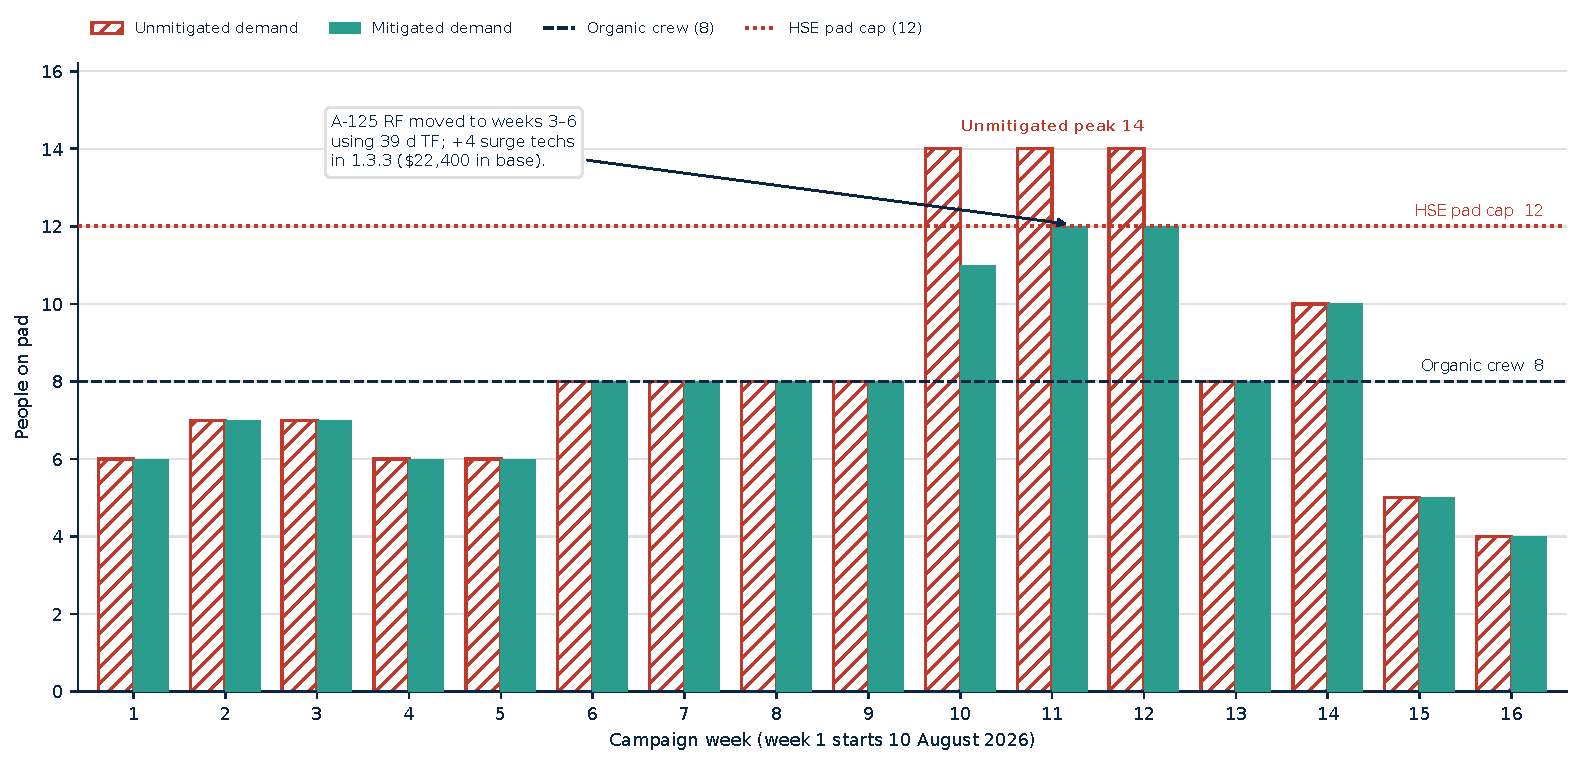
\includegraphics[width=0.98\linewidth]{resource_histogram.pdf}
\caption[Weekly pad demand versus capacity]{Weekly pad demand versus capacity, from Table~\ref{tab:resource-build}. Each bar is the maximum simultaneous unique-head count that week. Hashed crimson bars are the unmitigated series (peak 14 on 16--24~October): Wet Dress Rehearsal plus A-125 on its late bar plus four overtime heads. Teal bars are the mitigated baseline (peak 12): RF at $ES$--$EF$ in weeks 3--6, and four surge technicians on 24--30~October only. The navy dashed line is the organic crew of eight; the crimson dotted line is the HSE occupancy cap of twelve. Eight is not a hard pad limit.}
\label{fig:resources}
\end{figure}

% Generated by scripts/plot_resource_figures.py — do not edit by hand.
\begin{table}[H]
\centering
\footnotesize
\setlength{\tabcolsep}{3.2pt}
\caption[Weekly simultaneous pad occupancy]{Weekly simultaneous pad occupancy, from activity $\times$ named crew. Each weekly total is the maximum unique-head count on any calendar day that week (HSE cap is simultaneous, not weekly unique). Mitigated A-125 uses $ES$--$EF$; unmitigated uses the late bar $LS$--$LF$. Surge is four heads on 25--31~Oct only (7~days). Unmitigated overtime is four heads on WDR and static fire (16--30~Oct). Base, RF, surge and OT are disjoint name sets, so they add on the peak day.}
\label{tab:resource-build}
\begin{tabular}{@{}r l r r r r l r r r r@{}}
\toprule
Week & Mit.\ day & Base & RF & Surge & Mit. & Unmit.\ day & Base & RF & OT & Unmit. \\
\midrule
1 & 10~Aug & 6 & 0 & 0 & 6 & 10~Aug & 6 & 0 & 0 & 6 \\
2 & 17~Aug & 6 & 0 & 0 & 6 & 17~Aug & 6 & 0 & 0 & 6 \\
3 & 29~Aug & 6 & 2 & 0 & 8 & 24~Aug & 6 & 0 & 0 & 6 \\
4 & 31~Aug & 6 & 2 & 0 & 8 & 31~Aug & 6 & 0 & 0 & 6 \\
5 & 7~Sep & 6 & 2 & 0 & 8 & 7~Sep & 6 & 0 & 0 & 6 \\
6 & 14~Sep & 8 & 2 & 0 & 10 & 14~Sep & 8 & 0 & 0 & 8 \\
7 & 22~Sep & 11 & 0 & 0 & 11 & 22~Sep & 11 & 0 & 0 & 11 \\
8 & 28~Sep & 11 & 0 & 0 & 11 & 28~Sep & 11 & 0 & 0 & 11 \\
9 & 5~Oct & 11 & 0 & 0 & 11 & 7~Oct & 11 & 2 & 0 & 13 \\
10 & 12~Oct & 9 & 0 & 0 & 9 & 16~Oct & 8 & 2 & 4 & 14 \\
11 & 25~Oct & 8 & 0 & 4 & 12 & 19~Oct & 8 & 2 & 4 & 14 \\
12 & 26~Oct & 8 & 0 & 4 & 12 & 26~Oct & 8 & 0 & 4 & 12 \\
13 & 6~Nov & 5 & 0 & 0 & 5 & 6~Nov & 5 & 0 & 0 & 5 \\
14 & 15~Nov & 8 & 0 & 0 & 8 & 15~Nov & 8 & 0 & 0 & 8 \\
15 & 21~Nov & 4 & 0 & 0 & 4 & 21~Nov & 4 & 0 & 0 & 4 \\
16 & 23~Nov & 4 & 0 & 0 & 4 & 23~Nov & 4 & 0 & 0 & 4 \\
17 & 30~Nov & 4 & 0 & 0 & 4 & 30~Nov & 4 & 0 & 0 & 4 \\
\bottomrule
\end{tabular}
\end{table}


\subsection{Conflict resolution and fallback}
\label{sec:resource-escalation}

Resource conflicts escalate on the work, not on personalities. Tier~1 field leads have four hours to level, stagger or borrow from float without spending money. Tier~2 is the campaign PM: twelve hours to choose overtime, hire or resequence, with the cost consequence going to Ilsa so that Table~\ref{tab:wbs-cost} stays the book of record. Tier~3 is the Executive Board, with a 24-hour SLA, for any decision that consumes contingency or moves M-5 (30~October) or M-7 (15~November). Those gates are the same dates as Section~\ref{sec:schedule}; they are not a second calendar.

Team-member fallback is separate and is the A1 defect closed here. If a member is non-responsive for more than 48 hours, the Lead Planner audits the artefacts within 12 hours, the PM issues a WBS-reassignment addendum, and the Buddycheck PAF is locked against Teams and version history so that contribution evidence cannot be rewritten after the fact. That procedure reallocates packages in Table~\ref{tab:raci}; it does not authorise a silent change to $T$-0 or to $BAC$.


% -----------------------------------------------------------------------------
\section{Risk management}
\label{sec:risk}

Campaign risk is owned by Ziyad Alahmari (Risk and Quality Lead) and is scored on this pad, not as generic weather or budget-overrun rows. Eighteen cause--event--effect statements in Table~\ref{tab:risk-register} size the \$225{,}000 contingency already reported in Table~\ref{tab:contingency}, name the float that absorbs non-critical delay, and fix the owners who treat each item.

\subsection{Risk approach and scales}
\label{sec:risk-approach}

The process follows ISO~31000 identify--analyse--evaluate--treat--monitor \citep{iso31000}. Expected monetary value is calculated as in \citet{kerzner2017}: money is never read from the 1--5 heat-map scores. $EMV = P_{\%} \times I_{\$}$ uses the dollar column in Table~\ref{tab:risk-register}. Probability bands are $P=1$ below 5\% (3\% in EMV), $P=2$ from 5--20\% (12\%), $P=3$ from 21--40\% (30\%), $P=4$ from 41--60\% (50\%), and $P=5$ above 60\% (70\%). Schedule impact $I_{S}$ is 1 ($<2$~d), 2 (2--5~d), 3 (6--10~d), 4 (11--15~d) and 5 ($>15$~d on a $TF=0$ path). Cost impact $I_{C}$ is the dollar figure in the same row. The matrix coordinate $I$ is the maximum of those two bands \citep{pmi2021}. Residual $P$ and $I$ fall only where the named response actually bites. R-12 keeps $P=2$ because Option~C does not make the payload window more likely; it only prices the pull-in. Ziyad re-scores the register at Gate~1 (2~October), at M-4 (15~October) and at M-5 (30~October), in the same cadence as the EVM dashboard in Section~\ref{sec:delivery-evm}.

\subsection{Integrated risk register}
\label{sec:risk-register}

Table~\ref{tab:risk-register} is the full set. Cause, event and effect are three clauses. Owners match the RACI in Table~\ref{tab:raci}: Ziyad with the GSE Lead on static-fire abort (R-01) and township acoustics (R-17); the Launch Director on footprint and stage-separation (R-02, R-09); Ilsa Hashmi on LOX logistics, occupancy and the Juru commercial interface (R-10, R-13, R-04 with the Juru Cultural Officer); Hadi Alkhub on the dawn-lift window and countdown software (R-06, R-18); Abdul Wahab Obeid on permits, LRR deadlock and the Option~C draw (R-14, R-16, R-12). Figure~\ref{fig:risk-matrix} plots every inherent point and the residual after treatment. R-02 and R-09 share $(P,I)=(2,5)$ and are jittered so both remain visible.

\begin{figure}[H]
\centering
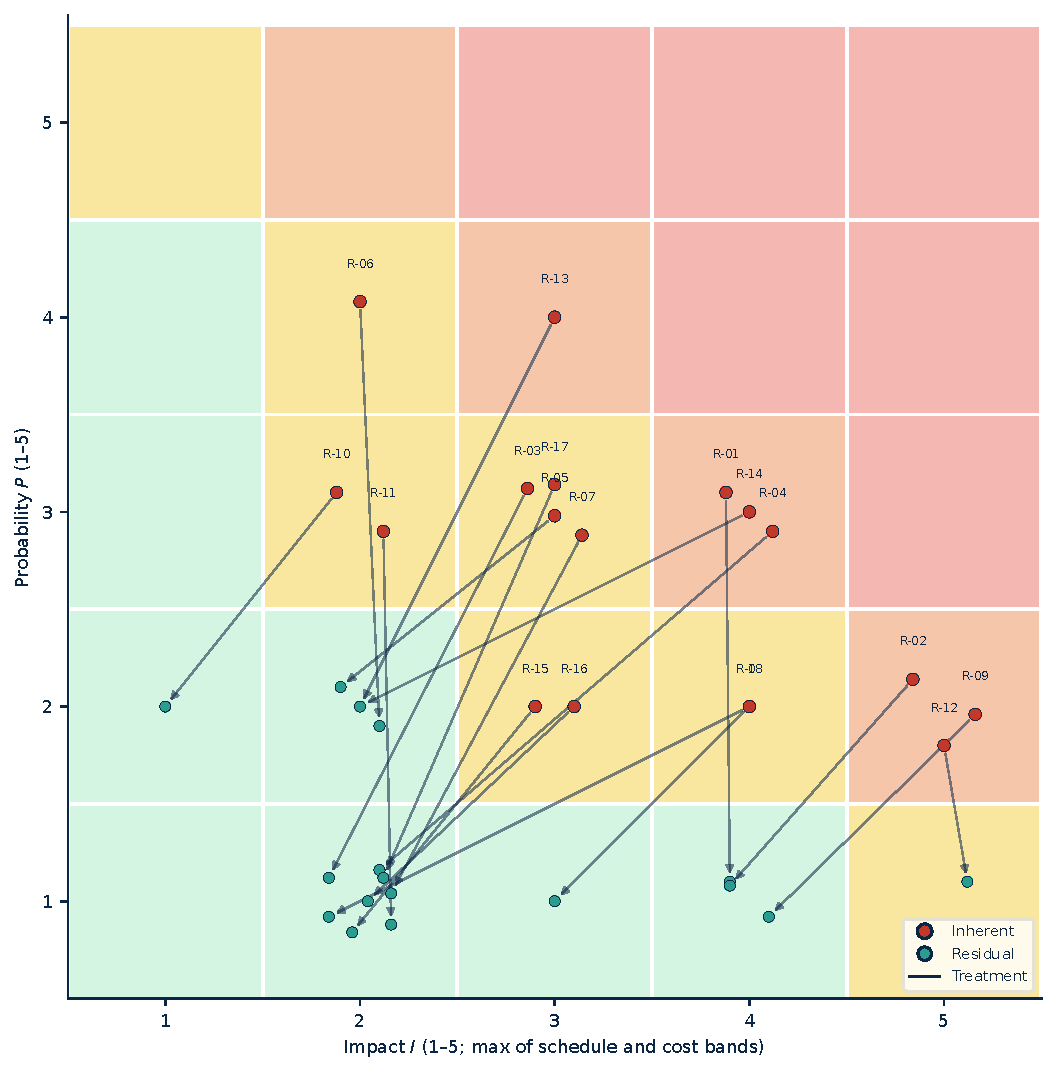
\includegraphics[width=0.82\linewidth]{risk_matrix.pdf}
\caption{Inherent (crimson) to residual (teal) movement for all eighteen register items. $P$ is vertical and $I$ is horizontal. Most treatment arrows run down and left. R-12 keeps $P=2$ (the payload window is not made less likely) and moves $I$ only. R-02 and R-09 share the $(2,5)$ cell and are offset.}
\label{fig:risk-matrix}
\end{figure}

\begin{landscape}
\footnotesize
\setlength{\tabcolsep}{3.0pt}
\renewcommand{\arraystretch}{1.12}
\begin{longtable}{@{}l l >{\raggedright\arraybackslash}p{4.55cm} c c c >{\raggedright\arraybackslash}p{2.28cm} >{\raggedright\arraybackslash}p{3.55cm} c c r@{}}
\caption{Integrated campaign risk register. $P{\times}I$ uses the 1--5 scores. EMV uses $P_{\%}\times I_{\$}$, not those scores. A dash means the row is not in the \$175{,}500 pool.}
\label{tab:risk-register}\\
\toprule
ID & Anchor & Cause $\rightarrow$ event $\rightarrow$ effect & $P$ & $I$ & $P{\times}I$ & Owner & Response & $P'$ & $I'$ & EMV \\
\midrule
\endfirsthead
\caption[]{Integrated campaign risk register (continued).}\\
\toprule
ID & Anchor & Cause $\rightarrow$ event $\rightarrow$ effect & $P$ & $I$ & $P{\times}I$ & Owner & Response & $P'$ & $I'$ & EMV \\
\midrule
\endhead
\bottomrule
\endfoot
R-01 & A-133 / 1.3.3 & Residual pump insulation $\rightarrow$ static-fire auto-abort $\rightarrow$ 12--14~d recycle / \$90k & 3 & 4 & 12 & Ziyad / GSE Lead & Thermal soak; on-pad LRU kit; 48~h recycle procedure & 1 & 3 & 27{,}000 \\
R-02 & A-143 / 1.4.3 & Trajectory energy toward park boundary $\rightarrow$ debris in GBRMPA zone $\rightarrow$ statutory halt & 2 & 5 & 10 & Launch Director & South-biased LRR footprint; joint GBRMPA protocol & 1 & 4 & 21{,}600 \\
R-03 & A-125 / A-143 & RF interference at Bowen array $\rightarrow$ telemetry $<$98.5\% $\rightarrow$ heritage fail & 3 & 3 & 9 & Avionics Lead & Dual-path recorders; A-125 before hot fire; mobile backup & 1 & 2 & 15{,}000 \\
R-04 & A-114 / A-143 & Exclusion without stop-work $\rightarrow$ Juru complaint $\rightarrow$ range withheld & 3 & 4 & 12 & Ilsa / Juru Officer & Embedded monitors with stop-work; cultural HP before A-132 & 1 & 2 & 12{,}000 \\
R-05 & A-124 / A-132 & Inadequate purge before LOX $\rightarrow$ frozen/cracked valve $\rightarrow$ WDR abort $\sim$8~d & 3 & 3 & 9 & GSE Lead & LN2 pre-chill; spare valve kit; helium leak test HP-2 & 2 & 2 & 16{,}500 \\
R-06 & A-123 / 1.2.2 & Abbot Point crosswind $>$20~kt at vertical mate $\rightarrow$ lift abort $\rightarrow$ crane standby & 4 & 2 & 8 & Hadi / Stack Conductor & Dawn-lift window; standby already inside 1.2.2 & 2 & 2 & 9{,}000 \\
R-07 & A-124 / D\&C & D\&C GSE IFC lags propulsion ICD $\rightarrow$ pad mismatch $\rightarrow$ rework & 3 & 3 & 9 & GSE Lead / PM & ICD freeze gate; weekly integration; D\&C LDs & 1 & 2 & 21{,}000 \\
R-08 & 1.2.3 / D\&C & Latent pad-civil defect $\rightarrow$ hold-down failure $\rightarrow$ hot-ops stop & 2 & 4 & 8 & D\&C mgr (A: PM) & NDT HP-1; defect liability remains with D\&C & 1 & 2 & 0$^{\ast}$ \\
R-09 & A-143 & Stage-sep charge timing error $\rightarrow$ debris outside footprint $\rightarrow$ inquiry / halt & 2 & 5 & 10 & Launch Director & Dual-string sep inhibit; wind hold toward park & 1 & 4 & 18{,}000 \\
R-10 & A-132 / 1.3.2 & Single 800~km LOX tanker delay $\rightarrow$ WDR cannot load $\rightarrow$ 2--5~d slip & 3 & 2 & 6 & Ilsa & 72~h tanker confirm; Townsville backup; RES on price & 2 & 1 & 6{,}900 \\
R-11 & A-131 & Flight-computer vs pad EGSE skew $\rightarrow$ power-on abort & 3 & 2 & 6 & Avionics Specialist & ICD freeze; cleanroom EGSE dry run before stack & 1 & 2 & --- \\
R-12 & A-143 & Payload LEO geometry valid only 10--12~Nov $\rightarrow$ board directs 5-day pull-in & 2 & 2 & 4 & Abdul / Sponsor & Pre-priced Option~C; draw \$21k from contingency if approved & 2 & 1 & --- \\
R-13 & A-132 / A-133 & Peak 14 vs cap 12 $\rightarrow$ detank error $\rightarrow$ recycle / injury & 4 & 3 & 12 & Ilsa & A-125 moved to Sep; four surge techs in base; 10~h stagger & 2 & 2 & 15{,}000 \\
R-14 & A-113 / A-143 & Townsville airspace / late NOTAM $\rightarrow$ 15~Nov slot refused & 3 & 4 & 12 & Abdul / Regulatory & File 60~d prior; weekly CASA liaison; Option~C backup & 2 & 2 & 13{,}500 \\
R-15 & A-142 & Dugong in exclusion box $\rightarrow$ sweep extension & 2 & 3 & 6 & RSO & Marine-mammal protocol; A-142 holds 4~d vs $T$-0 & 1 & 2 & --- \\
R-16 & A-141 & RSO vs Launch Director deadlock at LRR $\rightarrow$ missed 10~Nov gate & 2 & 3 & 6 & Abdul / Launch Director & Named DoA; escalate 24~h before A-141 $LF$ & 1 & 2 & --- \\
R-17 & A-133 & Static-fire acoustic $>$135~dB at Bowen $\rightarrow$ complaint / hold & 3 & 3 & 9 & Ziyad / HSE & Water deluge; 1.5~km exclusion; community notice 14~d prior & 1 & 2 & --- \\
R-18 & A-142 / A-143 & FTS/countdown abort at $T$-10 $\rightarrow$ recycle inside window & 2 & 4 & 8 & Hadi / Avionics & Two countdown rehearsals; abort-to-recycle procedure & 1 & 3 & --- \\
\end{longtable}

\vspace{0.3em}
{\footnotesize $^{\ast}$R-08 is contract-transferred (EMV \$0 to Gilmour). R-11, R-12, R-15--R-18 are schedule/HSE or priced only if Option~C is invoked. EMV identities: R-01 $0.30\times90{,}000$; R-02 $0.12\times180{,}000$; R-03 $0.30\times50{,}000$; R-04 $0.30\times40{,}000$; R-05 $0.30\times55{,}000$; R-06 $0.50\times18{,}000$; R-07 $0.30\times70{,}000$; R-09 $0.12\times150{,}000$; R-10 $0.30\times23{,}000$; R-13 $0.50\times30{,}000$; R-14 $0.30\times45{,}000$. Sum \$175{,}500.}
\end{landscape}

\subsection{Top risks, contingency, float and delivery model}
\label{sec:risk-response}

Three rows dominate board attention because they sit on the launch-critical path and can stop $T$-0 or close the range. They are not a recycled cyclone or ``budget overrun'' list. R-01 is a residual pump-insulation defect on A-133: auto-abort, a 12--14~day recycle, about \$90k of consumables. Ziyad and the GSE Lead treat it with thermal-soak instrumentation, an on-pad LRU kit and a 48-hour recycle procedure, which drops the score from $(3,4)$ to $(1,3)$ and leaves \$27{,}000 in the EMV pool. R-09 is a stage-separation timing error at A-143: debris outside the predicted footprint, GBRMPA inquiry, range halt. The Launch Director owns a dual-string inhibit and a wind hold toward the park; residual remains high-impact $(1,4)$ because a statutory halt does not become cheaper when the probability falls. R-02 is the sibling footprint risk (trajectory energy toward the park boundary) and is treated on the same LRR protocol; both remain Extreme-to-High on impact. R-14 is Townsville military airspace or a late NOTAM refusing the 15~November slot. Abdul files sixty days prior and holds a weekly CASA liaison. Crashing A-123 does not treat R-14: permits already finish on 24~October with $TF=0$, so a faster stack still waits on A-113. Option~C is the schedule backup, not a rewrite of the baseline.

Those eleven cost-bearing rows sum to \$175{,}500. Ilsa's RES allowance of \$49{,}500 covers in-scope LOX price variance, crane wind standby and unquantified pad anomalies. Together they are the \$225{,}000 in Table~\ref{tab:contingency}. Vehicle freight stays out of RES because it is out of scope. R-06 (Abbot Point crosswind at vertical mate) is a named lift-window risk owned by Hadi; its standby dollars already sit inside WBS~1.2.2, which is why the EMV is \$9{,}000 rather than a second crane line.

Float, not money, is the treatment for several feeders. A-125's 39 days let Ilsa park RF in weeks 3--6 so R-13 never meets an occupancy of 14. A-124's three days and A-114's five days absorb GSE and heritage delay before A-132 without moving 15~November. R-08 is transferred: the D\&C package manager remains Responsible, Abdul remains Accountable, and defect liability stays with the contractor after HP-1 NDT. R-12 is accepted on probability and pre-priced on cost. If the payload window is only 10--12~November, or if R-14 fires, Abdul takes Option~C to the Board and Ilsa draws \$21{,}000 from contingency. That draw is not in the \$1{,}500{,}000 work baseline, and it does not move the M-7 diamond on Figure~\ref{fig:gantt_chart} until the Board says so.


% -----------------------------------------------------------------------------
\section{Delivery and control}
\label{sec:delivery}

\subsection{Governance and reporting}
\label{sec:delivery-governance}
\emptysec

\subsection{Delivery model and procurement}
\label{sec:delivery-model}
\emptysec

\subsection{Quality}
\label{sec:delivery-quality}
\emptysec

\subsection{Health, safety and environment}
\label{sec:delivery-hse}
\emptysec

\subsection{Earned value management}
\label{sec:delivery-evm}
\emptysec

% -----------------------------------------------------------------------------
\section{Integration and professionalism}
\label{sec:integration}

\subsection{Document consistency}
\label{sec:integration-consistency}
\emptysec

\subsection{Presentation and referencing}
\label{sec:integration-presentation}
\emptysec

% -----------------------------------------------------------------------------
\section*{References}
\addcontentsline{toc}{section}{References}
\begin{thebibliography}{99}
\bibitem[Kerzner(2017)]{kerzner2017}
Kerzner, H. (2017). \textit{Project management: A systems approach to planning, scheduling, and controlling} (12th~ed.). John Wiley \& Sons.

\bibitem[Project Management Institute(2021)]{pmi2021}
Project Management Institute. (2021). \textit{A guide to the project management body of knowledge (PMBOK\textregistered\ guide)} (7th~ed.) and \textit{The standard for project management}. Project Management Institute.

\bibitem[SAE International(2016)]{sae2016}
SAE International. (2016). \textit{Quality management systems---Requirements for aviation, space, and defense organizations} (AS9100D). SAE International.

\bibitem[Rawlinsons(2025)]{rawlinsons2025}
Rawlinsons. (2025). \textit{Rawlinsons Australian construction handbook}. Rawlinsons Publishing.

\bibitem[Fair Work Ombudsman(2020)]{fwo2020}
Fair Work Ombudsman. (2020). \textit{Manufacturing and Associated Industries and Occupations Award 2020} (MA000010). Fair Work Commission.

\bibitem[Civil Aviation Safety Authority(2024)]{casa2024}
Civil Aviation Safety Authority. (2024). \textit{Cost recovery implementation statement: Aviation safety regulatory services}. Civil Aviation Safety Authority.

\bibitem[International Organization for Standardization(2018)]{iso31000}
International Organization for Standardization. (2018). \textit{Risk management---Guidelines} (ISO~31000:2018). International Organization for Standardization.
\end{thebibliography}

% -----------------------------------------------------------------------------
\appendix
\section{Contribution appendix}
\label{app:contribution}

\renewcommand{\arraystretch}{1.3}
\begin{tabularx}{\textwidth}{@{}>{\raggedright\arraybackslash}p{0.32\textwidth} >{\raggedright\arraybackslash}X r@{}}
\toprule
\textbf{Team member} & \textbf{Primary deliverables} & \textbf{\%} \\
\midrule
Abdul Wahab Obeid (s5303839) & Executive summary; integration; final QA & 25.0 \\
Hadi Alkhub (s5331680) & Scope; schedule; network logic; Gantt; compression & 25.0 \\
Ziyad Alahmari (s5375826) & Risk register; quality and HSE & 25.0 \\
Ilsa Hashmi (s5310047) & Cost; resources; capacity planning & 25.0 \\
\midrule
\textbf{Total} & & \textbf{100.0} \\
\bottomrule
\end{tabularx}

\vspace{1.4em}
\noindent
We confirm that the contribution percentages above are agreed by all members.

\vspace{1.4em}
\noindent
\begin{tabularx}{\textwidth}{@{}X X@{}}
Abdul Wahab Obeid \newline Signature: \underline{\hspace{4.2cm}} \newline Date: \underline{\hspace{3.0cm}}
&
Hadi Alkhub \newline Signature: \underline{\hspace{4.2cm}} \newline Date: \underline{\hspace{3.0cm}} \\[2.2em]
Ziyad Alahmari \newline Signature: \underline{\hspace{4.2cm}} \newline Date: \underline{\hspace{3.0cm}}
&
Ilsa Hashmi \newline Signature: \underline{\hspace{4.2cm}} \newline Date: \underline{\hspace{3.0cm}} \\
\end{tabularx}

\end{document}
